\documentclass[a4paper]{article}

%\usepackage{fullpage} % Package to use full page
\usepackage{parskip} % Package to tweak paragraph skipping
\usepackage{tikz} % Package for drawing
\usepackage{amsmath}
\usepackage{hyperref}
\usepackage[colorinlistoftodos]{todonotes}

\title{Lab 06-Textons and classifiers}
\author{Juan Carlos Leon Alcazar}
%\date{1984/02/14}

\begin{document}

\maketitle

\section{Description of the database}

The database\cite{Lazebnik2005} contains 1000 gray scale in JPG format, all of them have a standard 640x480 pixels resolution. Images are close ups of a given object surface, thus, containing textures found in different objects. There is a total of 17 classes \footnote{The object classes are: Bark Wood, Water, Granite, Marble, Floors, Pebbles, Wall Brick, Glass, Carpet, Upholstery, Wallpaper, Fur, Knit, Corduroy \& Plaid }, each contains between 30 to 90 sample images in the train set and between 10 to 30 images in the test set. Finally, there is a plain text file which specifies the naming convention for the images.


\section{Methodlogy}

Overall the mothodology used in this laboratory is presneten in figure ....

\begin{figure}[!ht]
	\centering
    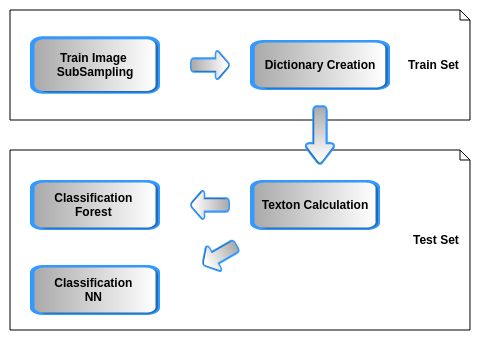
\includegraphics[width=0.95\textwidth]{img/Pipeline.png}
  	\caption{Elements of the proposed apporach}
\end{figure}

The original first step in the pipeline was the construction of a texton dictionary from the subset 'train'.  However, due to hardware constraints, it was not possible to build this dictionary with the complete train set (750 images). Creating a texton dictionary with a set of 40 images already requires about 45 GB of RAM memory (At peak), and about 3 hours CPU time. For the experiments, a single 115GB RAM machine was available. As it was not possible to create a dictionary with the full training set, it was reduced to 85 images (5 images per class).

There is not a clear way to subsample the original training set while retaining the original data variability, in other words, it is expected that this sub sampling process should create some bias in the dictionary. However the nature of the dataset might help to mitigate this issue: textures are essentially local patterns repeated, with some variability, at the global level. Thus it can be assumed that each image contains several instances of these local patterns, that already contain some of the variability of the texture.

To further test this hypotesis...  \todo{btreve experimento con 4 histogramas T1,5Imagenes T1n30I mages, T2n5Imagens,T2n30Imagenes, distancia chi-cuadrado}


\subsection{Textons}
After selecting the initial number of training images, there remains one final parameter for the construction of the texton dictionary, namely the K for the K means. For this matter we use a number of textons given by $K=c32$ ($c={1,2,3}$). The explanation behind this choice is that we expected the local patterns to closely match the shape of the filter bank; This is the case of c=1 $\rightarrow$ K=32. However, not every local pattern will match perfectly one of the textons on the filterbank. This is the case of $K={2,3}$ where the resulting clusters might contain the response information of several filters. No further values for $c$ are explored mostly, due to time constraints.
The final setup for the texton dictionary construction is the following:

\begin{itemize}
	\item Filter Bank: default filterbank provide in the implementations 16 orientations, 2 scales
	\item Number of training images: 85 (5 per each class)
	\item Number of clusters ($N$):  32, 64, 96
\end{itemize}

\subsection{Texton Calculation on Test Set}

With the 3 Texton dictionaries built we then calculate response of every image in the test set filtered with the obtained textons. for each image we obtain 3 responses (3 dictionaries) which are then represented by means of an histogram where the number of bins depends on the value of K used for the construction of the dictionary.

\subsection{Classification}
There are two methods selected for the classification of the textures

\begin{description}

\item[Nearest Neighbor] \cite{}
\item[Random Forest] \cite{}

\end{description}

The first methods has a single parameter: the distance metric, as specified by the assignment, we use the Chi-square distance to choose the Nearest Neighbour.

For the second method there are more parameters, the MATLAB implementation allows to choose:

\begin{itemize}
	\item Number of variables eligible for each decision split
	\item Cost of misclassifications
	\item Minimum number of observations per tree leaf
\end{itemize}

To allow for a maximum variability in the built trees we select the number of variables eligible for each decision split equals to the total amount of variables. Set the minimum number of observations to 1 and set no specific cost matrix for the experiments.

No adjustment is performed on the test data or the texton dictionary after being calculated.

Table \ref{table:table1} sumarizes the ruslts obtained for the Nearest Neighboug classifer:

NN
\begin{table*}[t]
\centering
\begin{tabular}{c | c | c}
Set Up & Precision & Recall   \\
\hline	
K=32 & 0.072 & 0.094 \\
K=64 & 0.1609 & 0.4667 \\
K=96 &  0.1163&  0.2553 \\

\end{tabular}
\caption{Precision and reacall for the Nearest neigborg classfifier}
\label{table:table1}
\end{table*}


Table \ref{table:table2}  sumarizes the results obtained for the Random Forest classifier:

20
\begin{table*}[t]
\centering
\begin{tabular}{ l | c | c}
Set Up & Precision & Recall   \\
\hline	
K=32,20 trees & 0.1159 & 0.2667 \\
K=64,20 trees & 0.1552 & 0.3000 \\
K=96,20 trees & 0.0789  &  0.2000 \\
K=32,50 trees & 0.1585 & 0.4333 \\
K=64,50 trees & 0.1458 & 0.3333 \\
K=96,50 trees &  0.1111 &  0.2333\\
K=32,100 trees & 0.1477 & 0.4333  \\
K=64,100 trees & 0.1687 & 0.4667  \\
K=96,100 trees & 0.1609 &  0.4667\\
K=32,500 trees & 0.1638 & 0.6333  \\
K=64,500 trees & 0.2072  &  0.7667 \\
K=96 & 0.1475 & 0.6000  \\

\end{tabular}
\caption{Precision and reacall for the Random Forest classfifier}
\label{table:table2}
\end{table*}


Overall both classifers perform very poorly on the test set. The Nearest Neigbourg classifier for K=32 has a performance similiar to that of random guess over the set of 17 classes. This behavior indicates that for K=32 the inter class distances in in the test set is very small and the class distribution does not follo an apprximate spatial pattern in in the space generated by the chi-square distance metric. 

For K=64 the result are similar forboth classifiers yet ther barely reach a 0.2 precision. This figure suggest that the clasisfier (either nearest Neighborgs or random forest) underperforms mostly due to a very high number of false positives. As can be confirme in table \ref{}. The random forest calssifer has a tendci to calssife most sample as belongi to clases 1 and 2 (bark and wood) and mostly ignores ever other class. 

Finally to confirm that the feature generation was the main problem and not the trainig process, we train an classify over the same subset (test). This yiesls a precision  of 1. and recall of 1.0 for the random forest with K=32. This indicate that the classifer can learn the patters presneted duirng the train time. However the pattern where not properly built




\bibliographystyle{plain}
\bibliography{bibliography.bib}
\end{document}

